\documentclass{article}
\usepackage{graphicx}
\usepackage{float}
\usepackage{hyperref}

\title{\textbf{TP Noté}}
\author{TROILLARD Romain \& RELAVE Dorian}
\date{\today}

\begin{document}

\maketitle

\tableofcontents

\newpage

\section{Analyse de l'évolution de la loss pendant l'apprentissage}

Nous avons analysé l'évolution des losses (train et test) lors de l'apprentissage d'un réseau de neurones sur le dataset MNIST. Les résultats sont présentés dans les graphiques suivants.

\subsection{Setup simple}

Pour ce setup, nous avons appliquer les fonctions telles quelle (entraînement sur un grand corpus et test sur un corpus plus petit)

\begin{figure}[H]
    \centering
    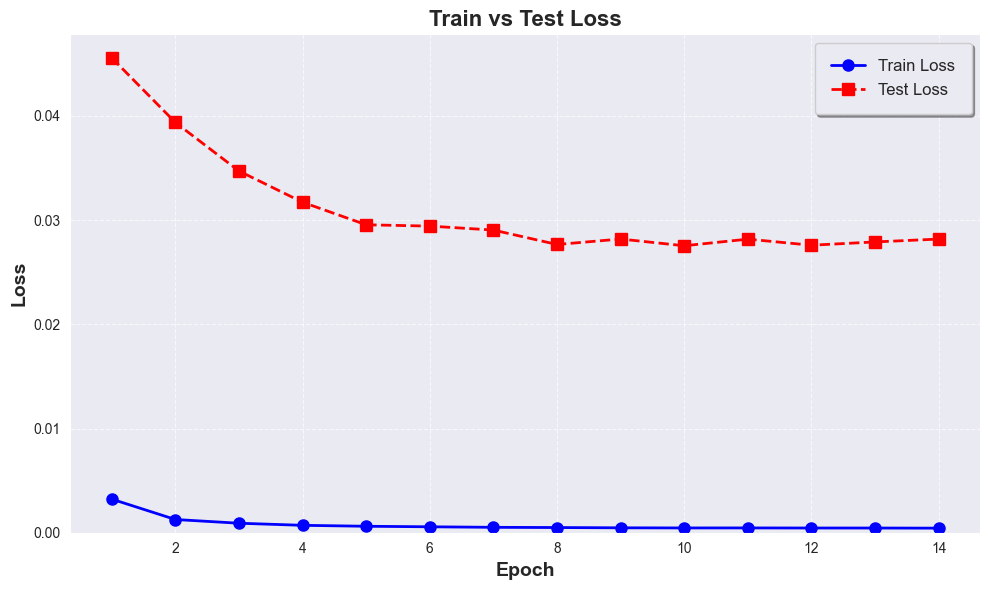
\includegraphics[width=1\textwidth]{train_vs_test.png}
    \caption{Évolution des losses (train et test) sur le setup de base}
    \label{fig:train_vs_test}
\end{figure}

On peut voir sur la figure \ref{fig:train_vs_test} que les deux courbes évoluent de façon décroissante et tendent vers 0 malgré une variation très faible à partir de la 5e epoch.

\newpage
\subsection{Setup inversé}

Pour ce 2e setup, nous avons appliqué les mêmes fonctions, mais nous avons inversé les données d'entrainement et de test (corpus test > corpus train).

\begin{figure}[H]
    \centering
    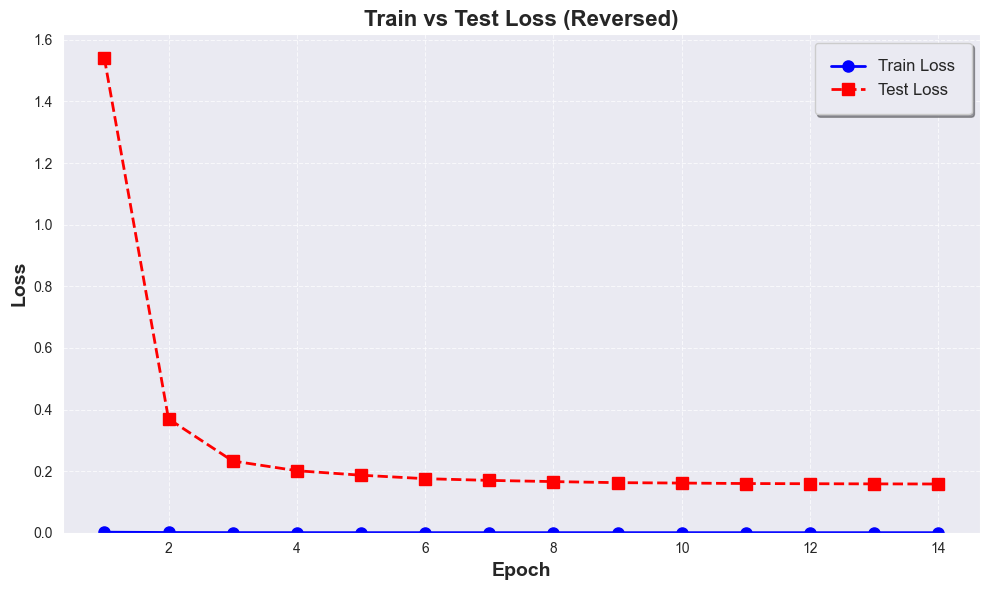
\includegraphics[width=1\textwidth]{train_vs_test_reversed.png}
    \caption{Évolution des losses (train et test) sur le setup inversé}
    \label{fig:train_vs_test_reversed}
\end{figure}

Ce second graphique (\ref{fig:train_vs_test_reversed}) nous montre une évolution similaire au setup de base, mais on voit une chute brutale entre la 1ere et la 2e epoch, cela est du au fait que la loss de la premiere epoch est particulierement élevé ce qui s'explique par la taille du plus petit jeu de données appliqué à l'entraienemnt

\newpage
\subsection{Setup sans 'Dropout'}
\label{Setup_nd}

Dans le cadre de ce 3e setup, il nous a été demandé de ne pas activer les fonctions 'Dropout' de la classe \textit{Net}.\\
Le \textbf{Dropout} est une technique permettant de réduire l’overfitting en supprimant temporairement des neurones et leurs connexions. 

\begin{figure}[H]
    \centering
    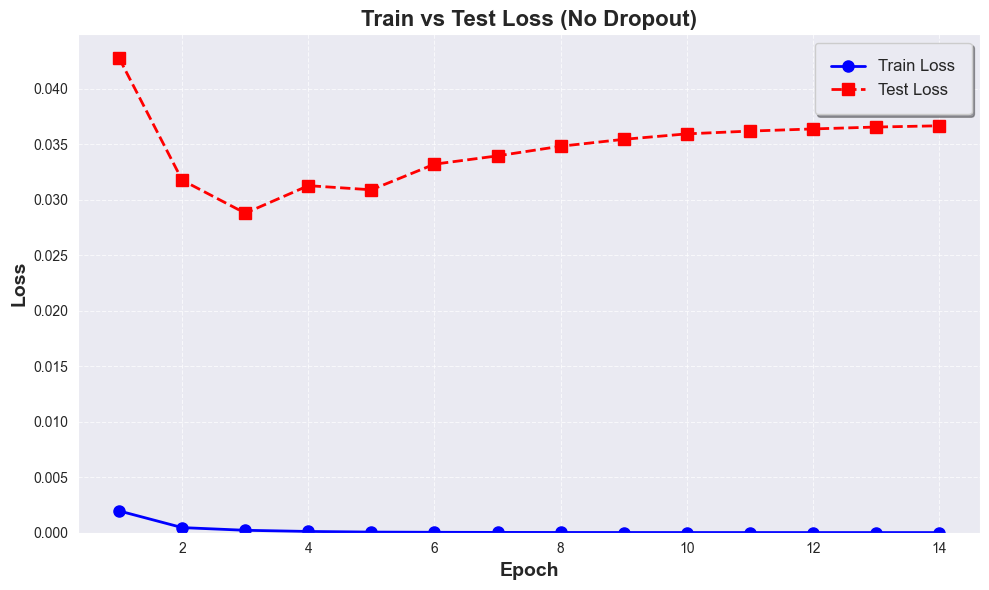
\includegraphics[width=1\textwidth]{train_vs_test_nd.png}
    \caption{Évolution des losses (train et test) sans dropout}
    \label{fig:train_vs_test_nd}
\end{figure}

Cette fois-ci sur le graphique \ref{fig:train_vs_test_nd}, on observe une situation différente, où la courbe \textit{train} tend vers 0 comme attendue, mais on voit sur la courbe \textit{test} que à partir de la 3e epoch, la loss augmente continuellement, ce qui nous informe d'un overfitting.

\newpage
\subsection{Setup inversée et sans 'Dropout'}

Pour ce 4e et dernier setup, on a désactivé le 'Dropout' et inversé les données d'entrainement et de test.

\begin{figure}[H]
    \centering
    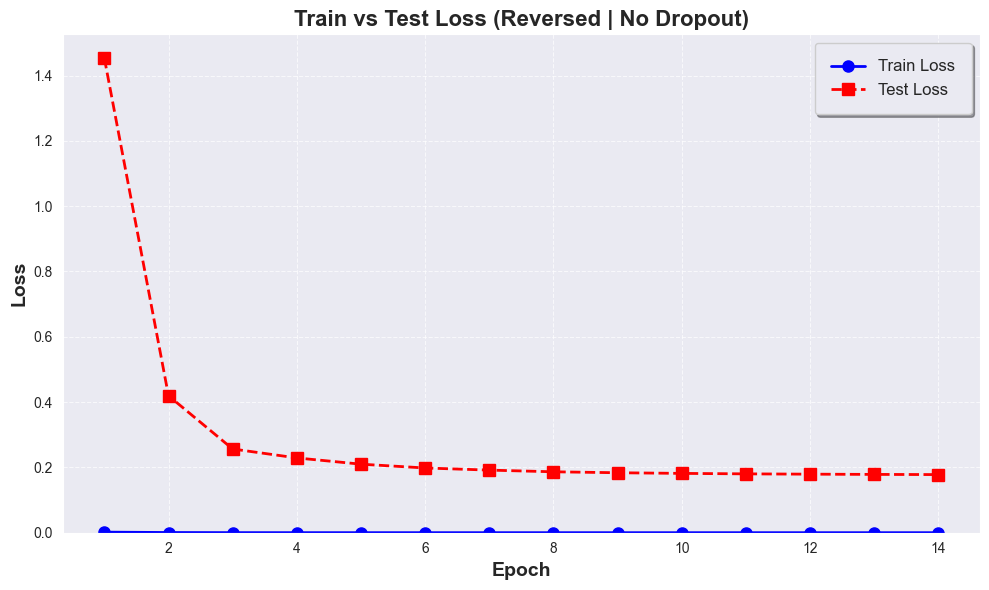
\includegraphics[width=1\textwidth]{train_vs_test_reversed_nd.png}
    \caption{Évolution des losses (train et test) inversée et sans dropout}
    \label{fig:train_vs_test_reversed_nd}
\end{figure}

Le graphique \ref{fig:train_vs_test_reversed_nd} est relativement semblable au graphique \ref{fig:train_vs_test_reversed} avec une loss importante sur la première epoch de test.

\newpage
\subsection{Conclusion}

Tout d'abord, nous allons comparer les différents setup

\begin{figure}[H]
    \centering
    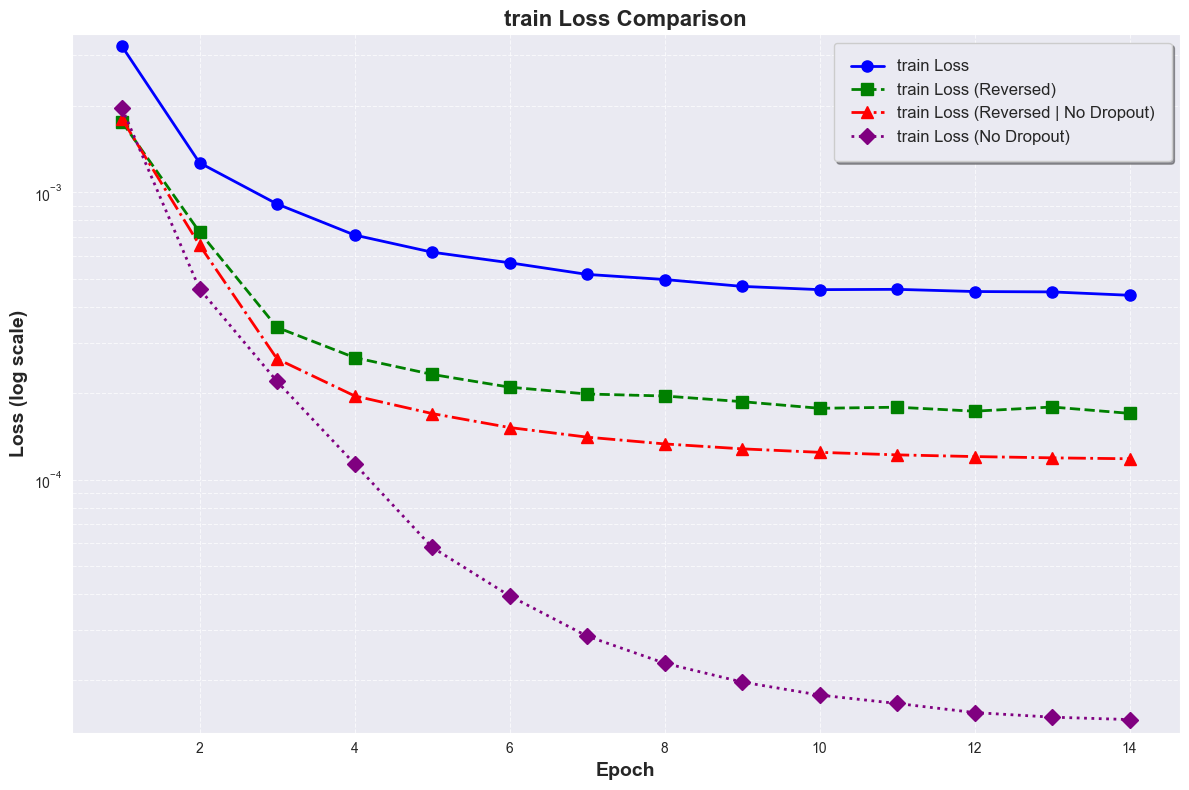
\includegraphics[width=1\textwidth]{train_compare.png}
    \caption{Évolution des losses train}
    \label{fig:train_compare}
\end{figure}

Les 4 courbes montrent que tous les setup ont une tendance décroissante de la loss sur la partie entrainement, les setup sans dropout ont des loss plus faible que les setup avec.

\begin{figure}[H]
    \centering
    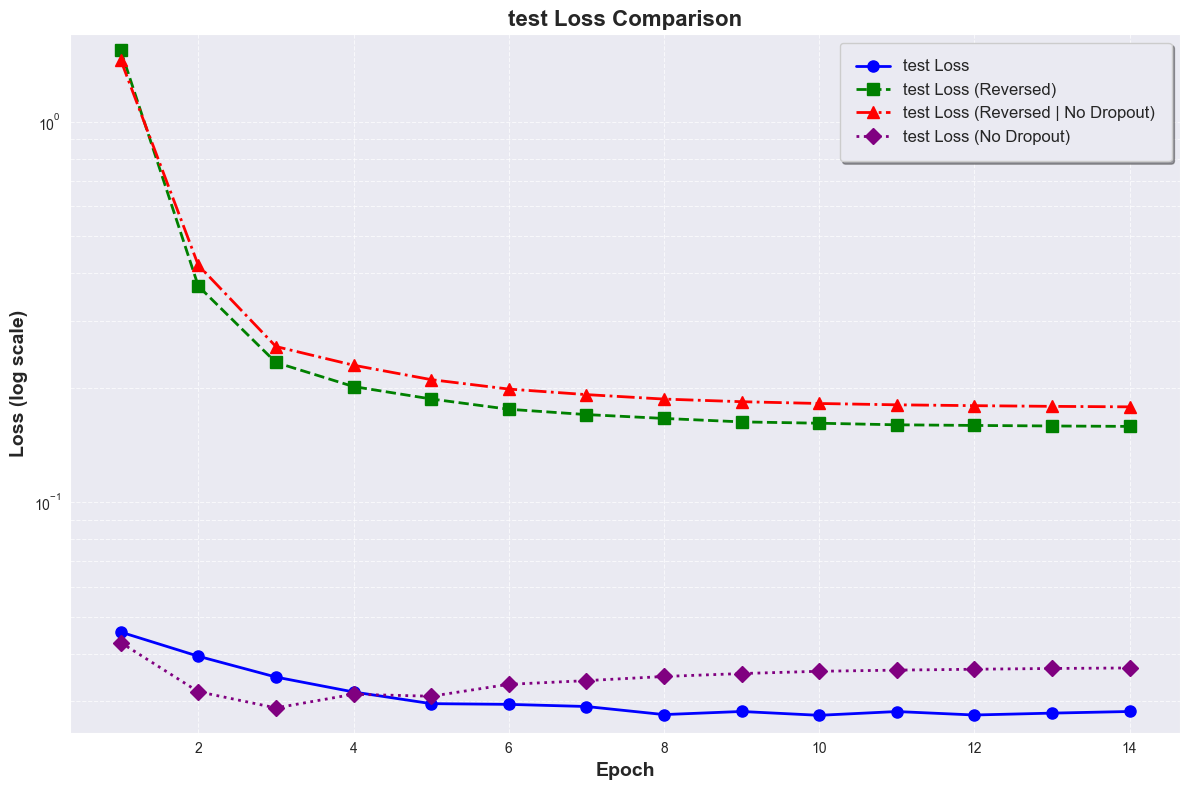
\includegraphics[width=1\textwidth]{test_compare.png}
    \caption{Évolution des losses test}
    \label{fig:test_compare}
\end{figure}

Pour la partie test, on observe un autre scénario avec les 2 setup inversé qui sont similaire avec une loss plus élevé que les setup non inversé. Enfin on remarque bien que le setup sans dropout prend une trajectoire montante contrairement au setup avec dropout qui tend vers 0. \\\\

En conclusion les différents setup nous montre que :

\begin{itemize}
    \item Lorsque le réseau apprend correctement, la loss sur le train diminue et tend vers 0.
    \item La loss de test suit généralement la même tendance, mais peut augmenter en cas de surapprentissage (comme dans le setup \ref{Setup_nd}).
    \item Inverser les données de test et d'entrainement n'est pas pertinent, car on obtient des loss plus élevé pour la partie test.
\end{itemize}


\end{document}